\chapter{Memory forensic in SGX environments}
\label{chp:forensic}


In this chapter, we take the role of a forensic analyst who is analyzing a copy 
of the physical memory acquired on an SGX-enabled machine. 
Many different variables can affect the analysis, including the way the memory 
image was acquired, the kernel drivers used to assist SGX operations, or the 
use of a certain SGX development framework. In this polyhedric scenario, we 
want to provide a clear guideline that helps a forensic analyst untangle the 
possible cases in an SGX-machine inspection. Our study shows which artifacts 
can be extracted in each case and discusses sound methodologies to extract those
artifacts.

We systematically evaluate our techniques in two different environments (a 
bare-metal machine and a VM in the Azure cloud) by using a set of $45$ SGX 
applications, a commercial SGX development framework~\citep{conclave}, and two 
state-of-the-art examples of malicious enclaves~\citep{sgxrop,snakegx}.
In all scenarios, our system was able to correctly detect and identify the
\emph{enclaves}, retrieve information about the
internal \emph{enclave} architecture, and identify their system interfaces
(\eg network communications or file-system access).
Furthermore, we discuss three practical use cases in which our techniques
can support an analyst to dissect a real application and two malicious 
\emph{enclaves}.

\vspace{0.2cm}
\noindent \textbf{Contribution.} In summary, we make the following 
contributions:
\begin{itemize}
	\item We discuss the limitation of current forensic analysis in 
	SGX-machines.
	\item We study which information can be extracted from a machine running 
	SGX \emph{enclaves} and propose new techniques to support their detection, 
	identification, and analysis (Section~\ref{sec:memory-forensic-sgx}).
	\item We evaluate our techniques on both open- and close-source projects, 
	and malware-enclave samples (Section~\ref{sec:memfor_evaluation}).
	Our open-source proof-of-concept tools are available 
	at \url{https://github.com/tregua87/sgx-forensic}.
\end{itemize}

\section{Threat Model}
\label{sec:system-assumptions}

In this work, we assume enclaves are correctly loaded in memory and
isolated from the other parts of the system thanks to the SGX technology.
In particular, we face two scenarios.
In the first case we assume that the enclave is operated by using a known
OS driver to handle the enclave pages and (for the user space analysis) the
application was developed by using a known SGX framework. 

In the second, more challenging, case, we remove these assumptions and consider
the case in which the analyst does not know the SGX drivers 
and has no information about the adopted development framework.

\section{Memory Forensic in SGX environment}
\label{sec:memory-forensic-sgx}

%\begin{figure}[t]
%	\centering
%	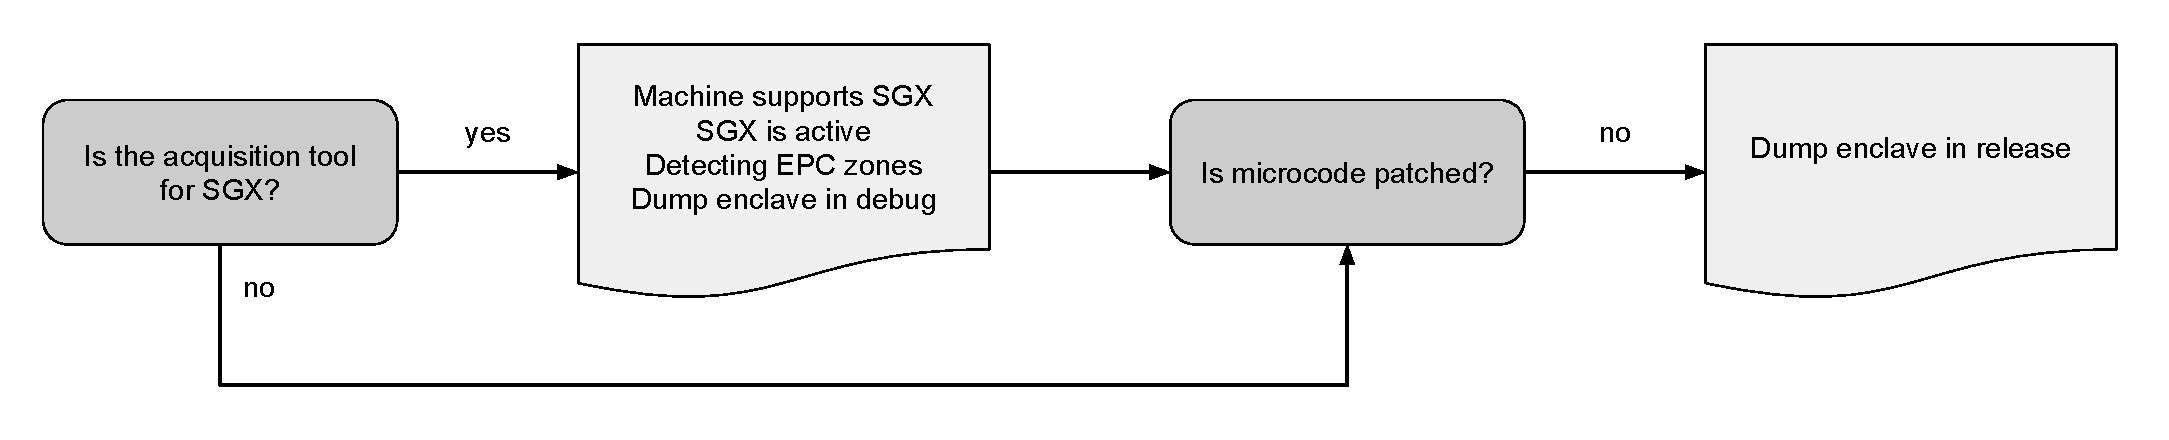
\includegraphics[width=\linewidth]{fig_c8/memory-acquisiton-map.pdf}
%	\caption{Mind map of memory acquisition.}
%	\label{fig:question-mem-aquisition}
%\end{figure}

\begin{sidewaysfigure}
	\centering
	%	\begin{minipage}{\linewidth}
	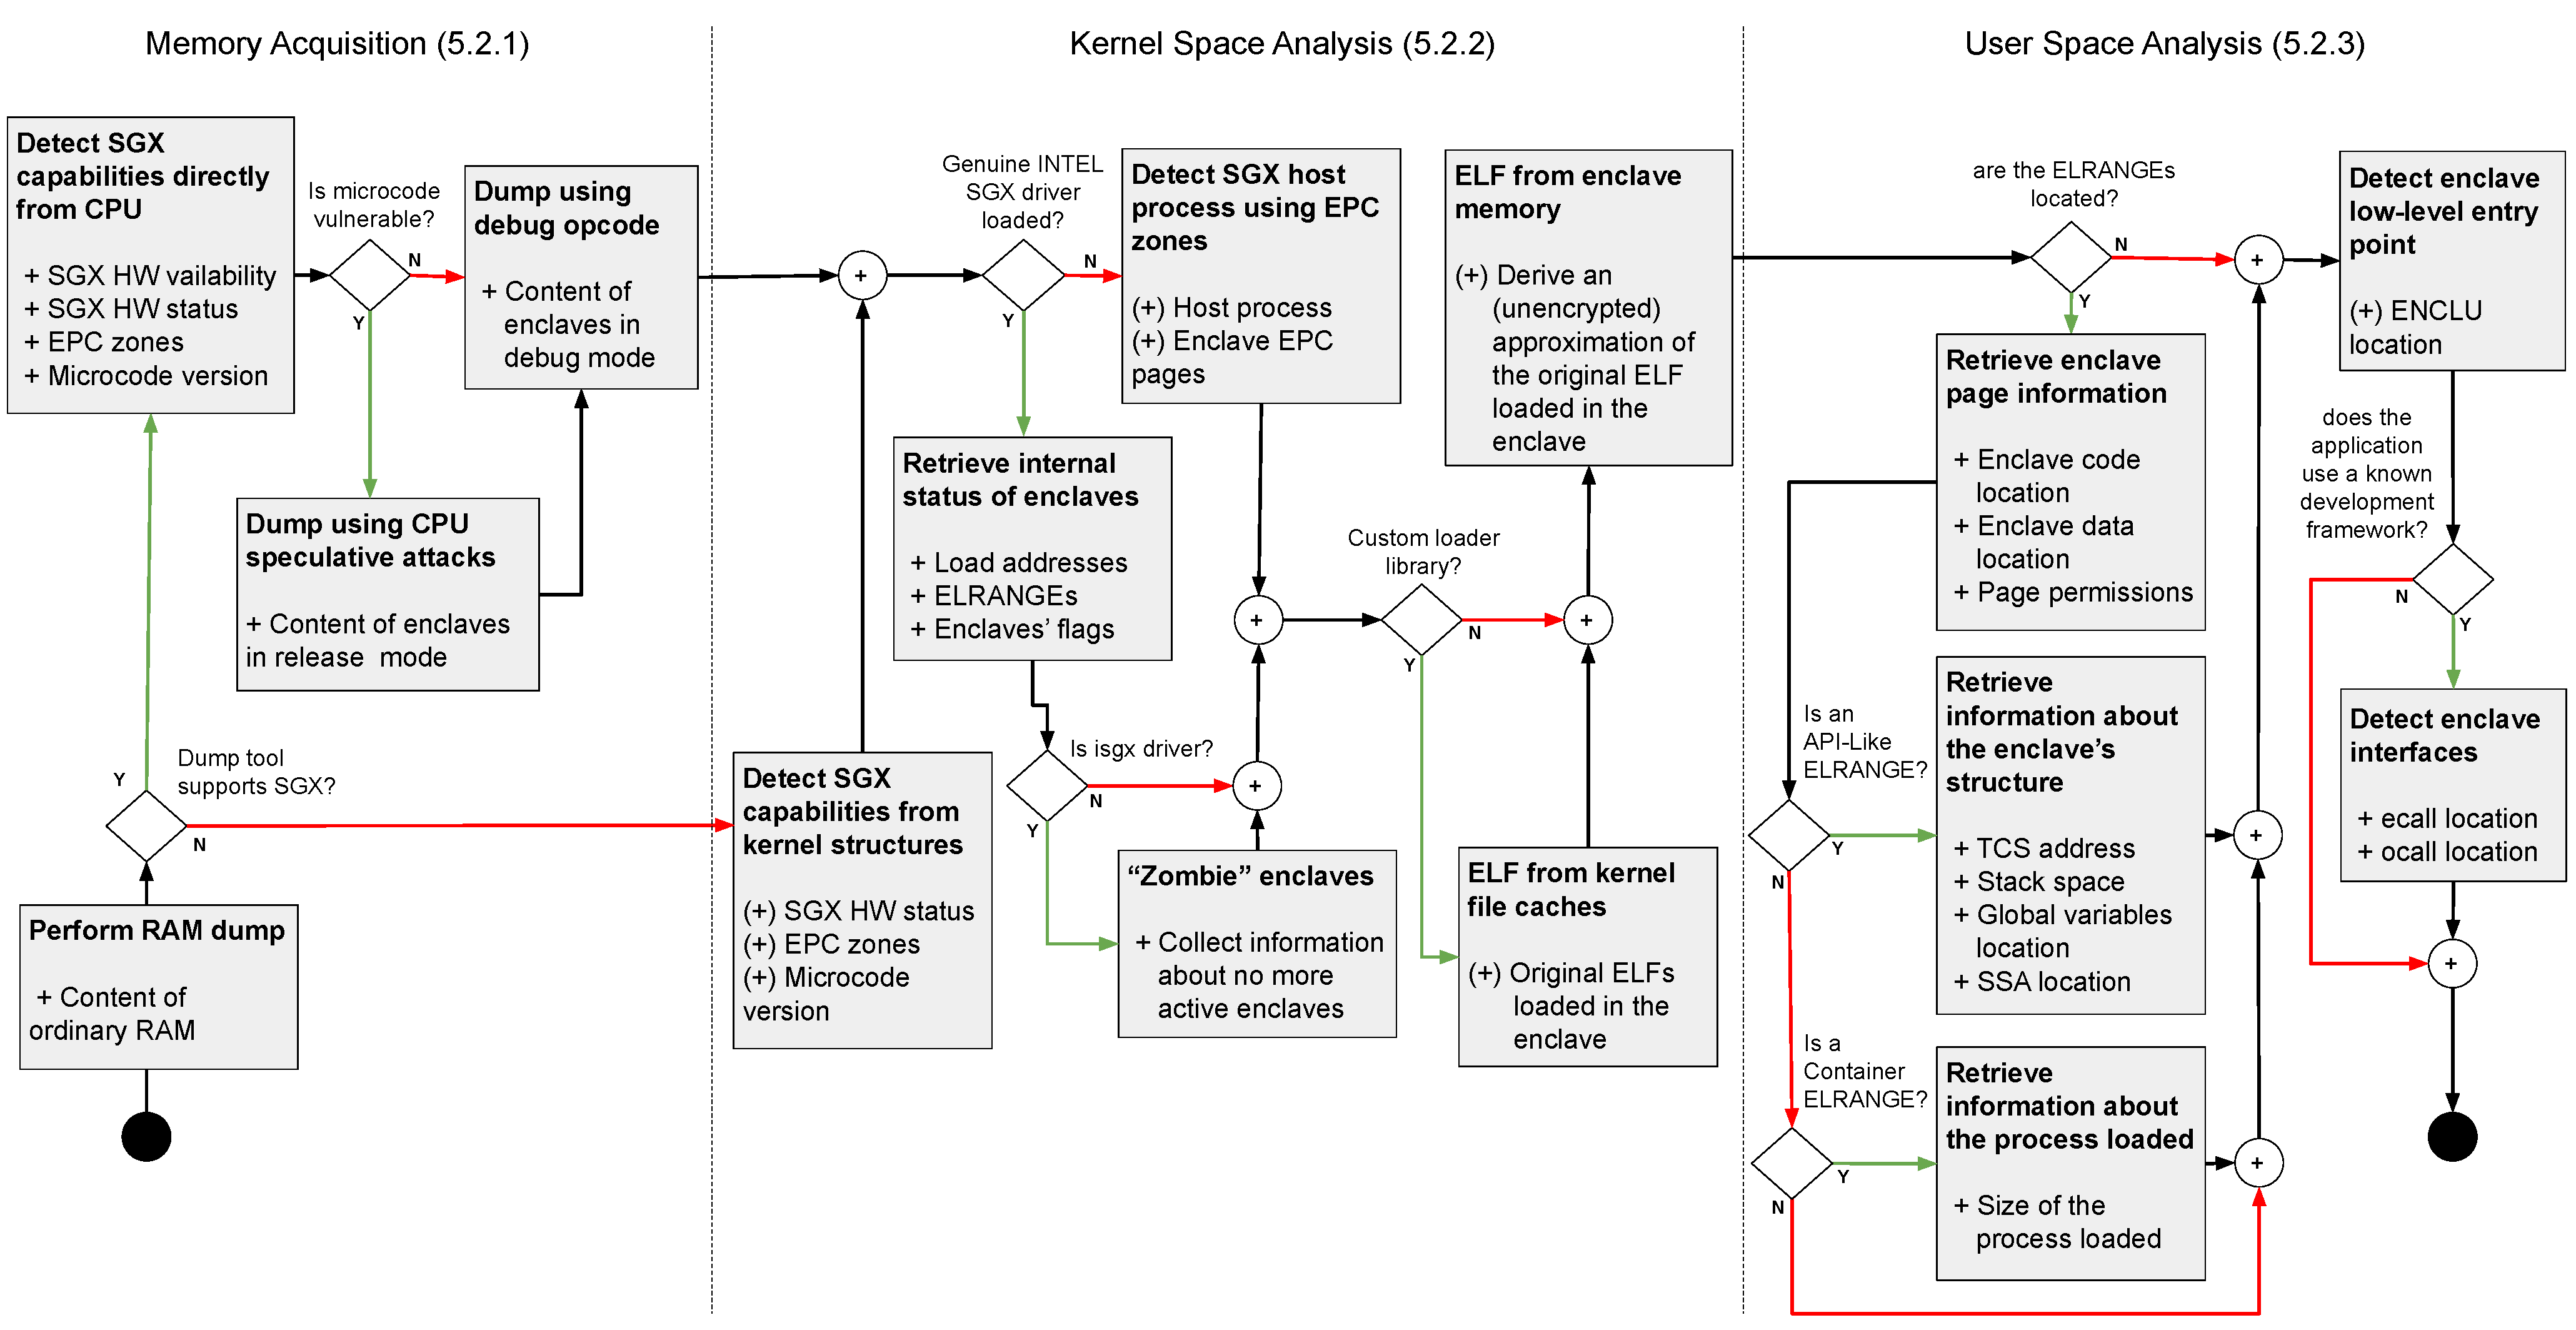
\includegraphics[width=\linewidth]{fig_c8/final_schema_sgx.pdf}
	\caption{The flowchart describes the workflow of an SGX-machine inspection 
		and depicts the three main phases: memory acquisition, kernel space, 
		and 
		user space analysis.
		The diamonds represent different conditions that can be 
		encountered (\eg \emph{Is microcode vulnerable?}), each condition leads 
		to 
		different class of information (\eg if the microcode is vulnerable, we 
		can 
		\emph{Dump using CPU speculative attacks}). Green-arrows with symbol 	
		``Y'' indicate the available information if a condition is satisfied, 
		while 
		red-arrows with symbol ``N'' otherwise.
		In addition, every box contains detailed pieces of information that we 
		mark 
		with the symbol ``$+$'' if they are always retrievable, while we use 
		the 
		symbol ``$(+)$'' if their availability depends by the system state (\eg 
		a 
		system log that might be wiped). 
		The technical details of each phase is detailed in their relative 
		section.}
	\label{fig:analysis-map}
	%	\end{minipage}
\end{sidewaysfigure}


%\textcolor{red}{
In this section, we tackle the various scenarios an analyst can face while 
inspecting an SGX-machine.
We split our study in three main phases: memory acquisition 
(Section~\ref{ssec:memory-dump}), kernel space analysis 
(Section~\ref{ssec:kernel-space-analysis}), 
and user space analysis (Section~\ref{ssec:user-space-analyses}).
For each phase, we discuss the possible conditions 
that an analyst can encounter, propose new analysis methodologies, and describe 
which information can be 
gathered from the system.
To clarify the different possibilities and provide a useful support for 
the analyst, we summarize the SGX forensics process into the flowchart in 
Figure~\ref{fig:analysis-map}.
The image contains all the scenarios discussed in our study and can serve
as a high-level guide for an SGX-machine inspection.
The map distinguishes, left to right, the three main phases described above 
(\ie memory 
acquisition, kernel-, and user-space analysis).
Each diamond identifies a different condition (\eg \emph{Dump tool support 
	SGX?}), while boxes synthesize the action that can be performed (\eg 
	\emph{Detect SGX 
	capabilities from kernel structures}) and the  
fine-grain information that can be recovered (\eg \emph{SGX HW 
	availability}). In this case, we use the symbol ``$+$'' to refer to a piece 
	of 
information always present, and the symbol ``$(+)$'' if the information might 
be present
(\eg a system log that might be wiped).
The details about each phase are described in the next sections.

\subsection{Memory Acquisition}
\label{ssec:memory-dump}

As explained in Section~\ref{sec:software-guard-extension}, each SGX enclave is 
composed of a set of encrypted physical pages which reside in an EPC memory 
zone. The CPU exposes the EPC memory zones as special MMIO devices not as part 
of the main memory of the system. For this reason, the OS does not include them 
in data structures that map all the ordinary memory regions available. However, 
the kernel is able to map EPC pages in the virtual-address space even if a 
direct read of their content returns a constant value (\ie \texttt{0xFF}) due 
to the SGX secrecy protections. Only when an enclave is running in debug mode, 
a kernel thread can dump the plain content of the enclave memory by using the 
special opcode \texttt{EDBGRD}. Ordinary dump tools, which relies on the 
operating system data-structures to identify available zones of the memory 
containing data, fail to find and dump the EPC zones. An SGX awared dump tool 
can overcome this limitation by querying
the CPU using the \texttt{CPUID} instruction~\citep{intel-developer-guide}, 
which permits to retrieve various configuration parameters including if SGX is 
present and enabled, all the EPC zones
defined on the system, their physical addresses, and sizes and the microcode
revision. It is important to note that this query to the CPU is based only on
opcodes and does not affects in any way the content of RAM, its
correctness, and coherency. 
Previous works that investigated malicious applications of SGX argued that, in 
practice, an adversary is incentivized to use enclaves in debug mode for 
deploying malware~\citep{zhang2018memory}.
This is because compiling an enclave in release mode requires to contact 
Intel, thus publicly exposing own identity.
Therefore we have developed a dump
tool which localizes the EPC zones, independently by the OS data-structures, 
marking them in the dump, and,
using \texttt{EDBGRD} opcode, saves pages related to debug-mode enclaves, 
without any information
on the number and exact location of them. This also permits to dump those
pages associated to past debug-enabled enclaves, which are not associated 
to a host process anymore.

% To this end, we have developed a modified version of the
% LiME~\cite{lime} kernel module able to identify all the EPC ranges available 
%on
% the machine (by using specific \texttt{CPUID} 
%leaves~\cite{intel-developer-guide})
% \ao{leaves it's the terminology used by Intel itself to define the various 
%branches used by CPUID opcode (it's a tree of subcommands)}
% and dump them. If the EPC zone contains pages belonging to a debug-enabled SGX
% enclave the module is able to retrieve their content. Otherwise, it returns a 
%page filled with
% \texttt{0xFF} bytes.
% By saving an entire EPC zone, without any information on the
% number and exact location of enclaves running in the system, also permits to 
%retrieve those
% pages associated to past debug-enable enclaves which are not associated 
%anymore with a
% host process.

% \db{we do not say that none of the existing tools dumps them and why. What is 
%the challenge?}

\vspace{0.2cm}
\noindent \textbf{CPU speculative attacks as forensics pinlock} --
% \ft{I guess this work should be included here Zhang et 
%al.~\cite{zhang2021see}}
% \ao{Zhang non e' adatto perche ricava informazioni sul comportamento dell 
%enclave ma non sul contenuto coerente della memoria, in pratica non dumpa 
%l'enclave a meno di non conoscere gia come funziona il suo codice, il che e' 
%un 
%controsenso.Gli attacchi a cui mi riferisco leggono l enclave senza sapere 
%nulla di come e' organizzata e quindi permettono di dumparle. In piu Zhang 
%sembra orientato alla difesa dell enclave che non e' il nostro caso}
Enclaves that run in release mode continue to be blind spots from the analyst
point of view. A possible way to dump the content of non-debug enclaves and
gaining a complete vision of the system status is to exploit CPU speculative
attacks. These classes of attacks, as summarized by \cite{nilsson2020survey},
allow an attacker to dump the content of an enclave even if it is not in debug
mode. In particular, \cite{vanbulck2018foreshadow} proposes 
Foreshadow-SGX and \cite{sgaxe} SGAxe, that permit to recover the content of 
the enclave with high accuracy in a finite time and without any knowledge of 
their internals. It is
important to note that all these attacks rely on CPU hardware bugs which are
quickly fixed by Intel through patched microcode updates. These updates are
fundamental to run enclaves which require remote attestation because in this
case attestation servers checks the microcode revision and only attests the
enclave if it is running on a fully-patched CPU. On the other hand, patched
microcode must be applied by the final users or released as BIOS updates by
motherboard producers and often require a machine reboot in order to be
enabled. System administrators of mission-critical servers, non-expert users and
unmanaged systems could delay the installation of patched microcode thus
permitting in certain cases to an SGX awared dump tool to exploit them to dump
also non-debug enclaves. In this case, the SGX-aware dump tool
can retrieve the microcode revision of the CPU by using the \texttt{CPUID} 
opcode, and if it is vulnerable to speculative attacks it can extract the 
content of enclaves running also in release mode.

\subsection{Kernel Space Analysis}
\label{ssec:kernel-space-analysis}

If the dump tool is not SGX-aware, no additional information about the SGX
configuration is collected from the machine at the acquisition time.
However, as shown in Figure~\ref{fig:analysis-map}, an analyst can deduct
these pieces of information by analyzing kernel data structures. For
example, it is possible to retrieve EPC zones by looking at the
\texttt{iomem\_resource} data structure, that contains MMIO mapped devices
(as shown in \texttt{/proc/iomem} on live systems). It is also possible to
extract logs lines from kernel logging facility (\texttt{dmesg}) in-memory
buffer. However, both data sources are not always available: early log
entries can be overwritten if the machine has a long uptime and some BIOS
vendor does not export EPC zones addresses as MMIO memory regions, making
them unavailable in \texttt{iomem\_resource}. 

When the status of the SGX hardware on the machine is not available, any
further analysis is more difficult and can result in a larger number of
false positives.

As explained in Section~\ref{sec:software-guard-extension}, SGX enclaves rely 
on the kernel to manage memory allocations: the kernel traces all pages 
allocated to the enclaves, assigns new ones when required, and evicts them when 
it no longer needs them. Furthermore, the kernel traces all the enclaves 
associated with a process and maps the enclaves' pages into the virtual address 
space of their host process. Non-monolithic kernels, as Linux and Windows, use 
specific drivers to manage enclaves. These drivers permit the user space 
enclave loader to the load the enclave pages inside the EPC memory. In 
particular, on Linux, there are two open-source drivers, developed by Intel, 
\texttt{isgx}~\citep{sgxdriver} and \texttt{DCAP}~\citep{sgxdcap}, which share 
very similar structure and functionalities. From a forensic perspective, the 
need of keep track of the enclaves status by the kernel allows to recover 
information on the enclaves present in a memory dump by analyzing the 
data-structures allocated by the kernel modules.

\begin{figure}[t]
	\centering
	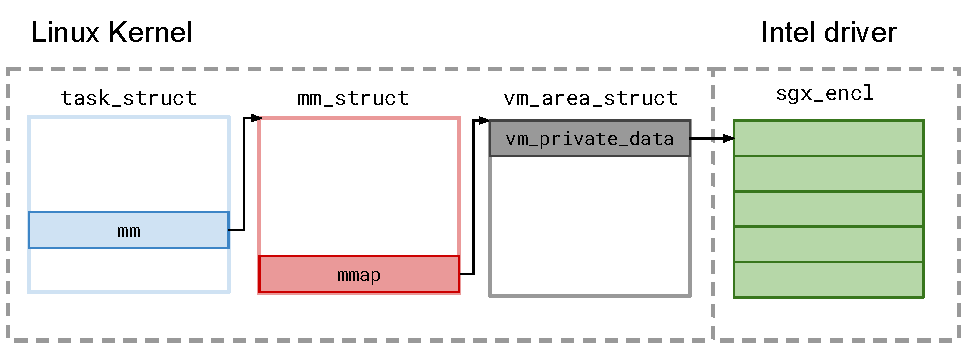
\includegraphics[width=0.8\linewidth]{fig_c8/sgx_driver}
	\caption{Relation between the kernel and Intel drivers data-structures}
	\label{fig:struct_sgx}
\end{figure}

Figure~\ref{fig:struct_sgx} shows the Intel drivers structures that handle the
enclaves pages. The drivers allocate private data-structures under the
\texttt{vm\_private\_data} space of the enclave's host process, which is
contained in an \texttt{vm\_area\_struct}. \newline
The \texttt{vm\_private\_data} contains information about the ELRANGE. The
\texttt{sgx\_encl} structures maintain:
\begin{enumerate*}[label=(\roman*)]
	\item the enclave load address,
	\item a list of the EPC pages allocated,
	\item the status flags of the enclave (\eg flags which indicate if an
	enclave is in debug mode, has performed cryptographic operations, the CPU
	capabilities required etc.) and,
	\item a linked list to the other enclaves instantiated on the system (this
	only for the \texttt{isgx} driver) which permits also to recover ``zombie''
	enclaves (\ie enclaves detached by the host process but not yet
	deallocated).
\end{enumerate*}

\vspace{0.2cm}
In the case in which the kernel uses a module unknown to the analyst, it is 
still possible
to rely on heuristics to determine the presence of an enclave in a process. In 
fact, the
enclaves pages have to reside in an EPC memory zone that is exposed by the CPU
as a separate hardware device, and the driver must threat it accordingly. For
example, on Linux systems, memory pages associated with MMIO devices, like SGX,
must be marked as \texttt{VM\_PFNMAP} and \texttt{VM\_IO}, which allows the
kernel to treat them in a special way with respect to ordinary memory 
operations. 
Therefore, to identify if a process has an associated
enclave, an analyst can check if it has memory pages flagged as part of special 
memory
zones without using any knowledge about the internal of the driver. Furthermore,
if the dump was performed by using an SGX-aware tool, it is also possible to
check if the candidate pages reside in an EPC zone to reduce false positives 
(\eg
processes which map common MMIO devices as graphic cards). However, this 
driver-agnostic
approach comes at a cost: it is not possible to determine the enclave base
address and its flags. These information are stored in the SECS page which is
not accessible, and can be recovered only if 
a copy is maintained into known driver data structures.

The code of an SGX enclave is distributed as dynamic library file (\texttt{.dll}
file under Windows and \texttt{.so} file under Linux). However, in contrast to
ordinary dynamic libraries, the enclave code is not loaded by the binary loader 
of the
system but it is loaded inside the memory enclave by an auxiliary dynamic
library. This process could leave,
in theory, various pieces of evidence in the kernel data structures.
For instance, caches
associated to the file descriptor of the loading library could contain traces of
the enclave code file.
However, the default library deployed
by Intel does not leave any trace of the original ELF loaded in the
kernel.
Furthermore, the security implementation of SGX offers a mitigation to the
possible information leaked due to the enclave loading 
(reducing the evidence from a forensics point of view): the code file containing
an enclave in release mode can be encrypted during the build, loaded inside the
enclave and decrypted only inside the protected memory~\citep{sgx-cypher}. 

However, if we have performed a dump with an SGX-aware tool, we can reconstruct
the ELF file loaded into the enclave starting from the content of the enclave
itself. This permits, if the dump also contains pages of enclaves in release
mode, to bypass the encryption technique used by the author to hide the content
of the ELF file loaded  since we extract the decrypted version of the ELF
directly from the enclave memory.

\subsection{User Space Analysis}
\label{ssec:user-space-analyses}

Since enclaves need a user-space component to interact with the system,
an analyst can gather information by analyzing structures that reside 
in the untrusted memory of user-space processes.
In particular, we discuss the recovery of the enclave memory layout and the 
enclave interface.

\subsubsection{Enclave Memory Layout Analysis}

\begin{figure}[t]
	\centering
	\begin{subfigure}[t]{0.49\linewidth}
		\centering
		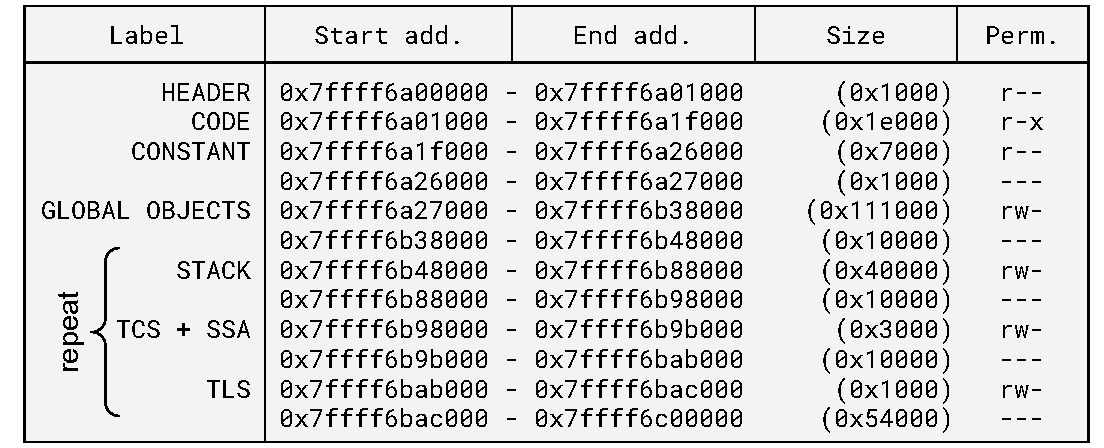
\includegraphics[width=\textwidth]{fig_c8/memory_layout_api}
		\caption{Example of Memory layout of\\Intel SGX SDK.}
		\label{fig:memory_layout_api}
	\end{subfigure}
	\hfill
	\begin{subfigure}[t]{0.49\linewidth}
		\centering
		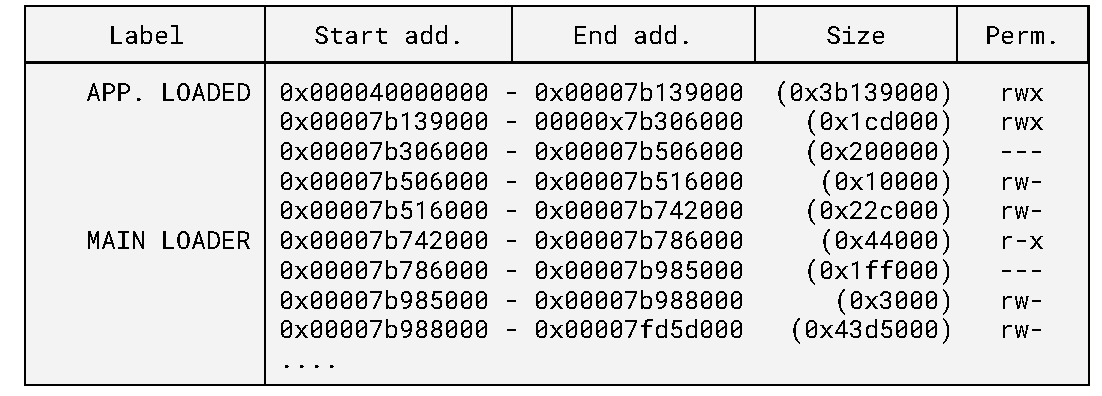
\includegraphics[width=\textwidth]{fig_c8/memory_layout_container}
		\caption{Example of Memory layout of Graphene.}
		\label{fig:memory_layout_container}
	\end{subfigure}
	\caption[Memory layout example.]{Memory layout example for API-like and 
	Container-like frameworks.}
	\label{fig:memory_layout}
\end{figure}

It is possible to infer 
the enclave memory layout by inspecting the page permissions of its ELRANGE. 
The Intel documentation proposes a well-defined internal layout that helps 
defining multi-thread enclaves and is thus adopted by all the API-like 
frameworks we analyzed. 
However, the enclave memory layout is quite flexible, as in the case of the 
Container-like frameworks. We implemented an algorithm that is able to analyze 
the enclave memory layout and automatically infers if the framework is an 
API-like, a Container-like, or none of them.
In Figure~\ref{fig:memory_layout}, we exemplify an API-like and a 
Container-like framework.
Below, we describe what information can be gathered in the two scenarios
and we discuss what can be done when the enclave does not follow any known 
structure.

\vspace{0.2cm}
\noindent \textbf{API Like} -- All the API-like frameworks that we studied 
follow the
standard Intel SGX SDK layout, which is exemplified in
Figure~\ref{fig:memory_layout_api}. This layout does not have \texttt{rwx}
pages by default and it expects as first pages respectively the enclave header, 
the code,
constants, and the global objects (\eg BSS or heap data). The rest of
the memory is dedicated to the trusted threads~\citep{intel-developer-guide}. In
particular, a trusted thread is composed of four parts:
\begin{enumerate*}[label=(\roman*)]
	\item the stack space,
	\item the Thread Control Structure (TCS),
	\item a fixed number of State State Area (SSA), and
	\item the Thread-Local Storage (TLS)
\end{enumerate*}.
The same structure is repeated for each trusted thread.

TCSs are particularly important because they are used as input for
\texttt{ENCLU}. Moreover, modern SGX threats use TCS addresses for ROP-chains 
that interacts with the enclave~\citep{snakegx}. 
Therefore, inferring the TCSs is crucial for an analyst to identify such 
threats in memory.

\vspace{0.2cm}
\noindent \textbf{Container-like} -- This second type of enclaves usually 
adopts custom layouts
that are designed to host whole applications, as shown in
Figure~\ref{fig:memory_layout_container}. These frameworks also contain
libraries to simulate an operating system~\citep{tsai2017graphene} and allocate 
one or more \texttt{rwx} blocks for the loaded application.
Due to the custom nature of these frameworks, we cannot infer important
structures, such as TCSs. However, an analyst can estimate the size of the 
loaded application
by measuring the size of the \texttt{rwx} area.

\vspace{0.2cm}
\noindent \textbf{Unknown} -- 
If the enclave does not fall in the previous two classes, the information that 
can be
extracted in an automated fashion is very limited. However, it is still 
possible to gather
few clues by observing the page permissions.
For instance, an analyst can locate and measure the size of executable pages, 
which reveals 
the amount of code loaded in the enclave.
Moreover, it is possible to enumerate writable pages (\ie \texttt{rw*}), that 
likely point to data
location.

\subsubsection{Enclave Interface Analysis}

The \emph{enclave} interface reveals the type of interaction with the 
underlying OS.
However, the \emph{enclave} interface strictly depends from the adopted 
development 
framework.
To this end, we compiled a list of framework fingerprints composed by 
specific tokens, list of loaded libraries, and name patterns of the main 
ELF file used. By using these signatures, it is possible to identify the 
framework
and retrieve the interface information.

In case the framework is unknown, such as for a custom 
SGX malware, there is no automatic way to infer the enclave interface. 
However, the host process still requires to invoke an \texttt{ENCLU} opcode to 
interact with the enclave (Section~\ref{sec:software-guard-extension}).
This reveals the low-level entry-point of the enclave, which serves as starting
location for the analyst to manually reverse engineer the enclave interface.

In case of a known development framework, instead, we propose an 
automatic interface extraction that is based on a combination of memory 
forensic and reverse engineering techniques, with a similar approach of what 
\cite{grazianohyper} implemented for the analysis of hypervisors.
Overall, our analysis is composed of two steps. First, we locate meaningful
structures inside a memory dump (\eg \emph{outside functions} are organized as
an array of function pointers). Then, we apply a lightweight static analysis 
phase to identify the
usage of such structures (\eg the function \texttt{sgx\_ecall} accepts an array
of function pointers as third parameter). This approach 
is sound, because the code is automatically generated by the
framework and thus follows predictable patterns.

It would also be possible to employ more sophisticated semantic software 
similarity techniques~\citep{pei2020trex}. However, due the nature of the 
\emph{edge} component, we argue that static approaches best suit our scenario.
And in fact, our static analysis solution resulted in zero false positive and 
zero false negative in our experiments (Section~\ref{ssec:correctness}).
In the following, we provide some examples on how we recognize \emph{outside} 
and \emph{secure functions}, respectively.

Our approach is based upon two observations. First, important functions (\eg 
\emph{outside functions}) are always organized in an array of function pointers 
(\eg \emph{ocall\_tables}). 
Second, the location of these structures is hard-coded in 
crucial utilities.
This allows us to automatically locate the usage of
this structure in the code by checking the signature of known functions.
For instance, in case of the Intel SGX SDK, \texttt{sgx\_ecall} functions 
expects a pointer to an \emph{ocall\_table} as third parameter (\ie the register
\texttt{rdx} for Linux $64$).
Moreover, the \emph{secure functions} (in  Intel SGX SDK) always invoke 
\texttt{sgx\_ecall} from an external library (\texttt{libsgx\_urt.so}), thus 
importing the symbol.
Therefore, locating the invocations points to \texttt{sgx\_ecall} reveals 
both \emph{outside} and \emph{secure functions}.
In Section~\ref{apx:interface-analysis}, we detail the algorithm used.

Recovering the enclave interface is important when the enclave content is
inaccessible (\eg the enclave is in release mode). 
For instance, an analyst might find an undocumented enclave in the system (\eg 
a malware-enclave) and he is interesting in studying its behavior.
In this case, the \emph{secure functions} indicate the 
data accepted by the enclave, \eg buffers, pointers to the untrusted memory. 
The \emph{outside functions}, instead, represent the interaction with 
the system, \eg writing files, network communication.
The combination of \emph{outside} and \emph{secure functions}, therefore, can 
give an intuition of the internal enclave logic.

\section{Interface Analysis Algorithms}
\label{apx:interface-analysis}

These are the pseudo-code used to extract either \emph{secure} and 
\emph{outside functions} from a process memory dump.
The Algorithm~\ref{alg:interface-sgxsdk-rustsgx} shows our approach for the 
Intel SGX SDK and RUST-SGK, the Algorithm~\ref{alg:interface-openenclave} shows 
our approach for Open Enclave SDK, and finally the 
Algorithm~\ref{alg:interface-graphene-sgxlkl} shows our approach for Graphene 
and SGX-LKL.

\subsection{Intel SGX SDK and RUST-SGX}
Alg.~\ref{alg:interface-sgxsdk-rustsgx} describes the approach for these two
frameworks.
In particular, we exploit the fact that the host application imports the
symbols \texttt{sgx\_ecall} from \texttt{libsgx\_urts.so}.

In the algorithm, we first create a list of \emph{ecall}
(line~\ref{alg:sgxsdk:2}) and confirmed \emph{ocall\_table}s
(line~\ref{alg:sgxsdk:3}); that will contain the enclave interfaces.
Then, we extract a list of possible \emph{ocall\_tables} from the \texttt{r--}
and \texttt{r-x} pages of the ELF extracted from memory 
(line~\ref{alg:sgxsdk:4}).
We consider possible \emph{ocall\_tables} any list of addresses (\ie sequence
of $8$ bytes) that point to \texttt{r-x} pages of the main ELF.
In the rest of the algorithm, we apply a static analysis pass on the code
scanning all functions (line~\ref{alg:sgxsdk:5}).
Our goal is to identify those functions $f$ that invoke \texttt{sgx\_ecall} by
using one of the possible \emph{ocall\_table} as parameter
(line~\ref{alg:sgxsdk:7}).
% Since we deal with Linux $64$bit machines, we except that the
% \emph{ocall\_table} is assigned to the register \texttt{rdx}.
Once we locate a function that satisfies our requirements, we save the function
$f$ in \emph{ecall\_list} and its \emph{ocall\_table} in
\emph{ocall\_table\_conf} (lines~\ref{alg:sgxsdk:8} and~\ref{alg:sgxsdk:9}).
Finally, we return \emph{ecall\_list} and \emph{ocall\_table\_conf}
(line~\ref{alg:sgxsdk:11}).

\subsection{Open Enclave SDK}
Alg.~\ref{alg:interface-openenclave} describes the approach for Open Enclave
SDK.
In this case, the framework identifies the \emph{secure functions} through
string tokens that are grouped in an array of strings, called
\emph{ecall\_tokens}.
% We thus integrate a similar approach than \emph{ocall\_table}.

In the algorithm, we first create a list of \emph{ecall}
(line~\ref{alg:open:2}) and confirmed \emph{ocall\_table}s
(line~\ref{alg:open:3}); that will contain the enclave interfaces.
Moreover, we create a list of \emph{ecall\_tokens\_conf}
(line~\ref{alg:open:4}).
At this point, we extract a list of possible \emph{ocall\_tables}
(line~\ref{alg:open:5}) and a list of possible \emph{ecall\_tokens}
(line~\ref{alg:open:6}) from the \texttt{r--} and \texttt{r-x} pages of the
main ELF.
We consider possible \emph{ocall\_tables} any list of addresses (\ie sequence
of $8$ bytes) that point to \texttt{r-x} pages of the main ELF.
Moreover, we consider possible \emph{ecall\_tokens} any array of
null-terminated ascii strings.
In the rest of the algorithm, we statically analyse all functions
(line~\ref{alg:open:7}).
to identify those functions $f$ that invokes
\texttt{oe\_create\_enclave}, the function used to create an enclave.
In particular, \texttt{oe\_create\_enclave} expects an \emph{ocall\_table} as
8th parameter (pushed into the stack) and \texttt{ecall\_token} as third
parameter (line~\ref{alg:open:9}).
Once we locate a function that satisfies our requirements, we save the
\emph{ocall\_table} in \emph{ocall\_table\_conf} and the \emph{ecall\_tokens}
in \emph{ecall\_tokens\_conf} (lines~\ref{alg:open:10} and~\ref{alg:open:11}).
The \emph{ecall\_tokens} are also used in the actual \emph{secure function}
invocation.
We thus scan the functions and select those that have a pointer to one of the
\emph{ecall\_tokens\_conf} elements (line~\ref{alg:open:13}
to~\ref{alg:open:15}).
Finally, we return \emph{ecall\_list} and \emph{ocall\_table\_conf}
(line~\ref{alg:open:17}).


\subsection{Graphene and SGX-LKL}
Alg.~\ref{alg:interface-graphene-sgxlkl} describes the approach for these two
frameworks.
In this case, the enclave exposes \emph{one} secure function that boots
the application loaded into the enclave.

In the algorithm, we list the functions that contain the \texttt{ENCLU} opcode
in the main ELF memory space (line~\ref{alg:cont:2}).
The \texttt{ENCLU} plays the role of \emph{ecall} for the enclave.
Then, we create a list of confirmed \emph{ocall\_table}s
(line~\ref{alg:cont:3}) and extract a list of possible \emph{ocall\_tables}
from the \texttt{r--} and \texttt{r-x} pages of the main ELF
(line~\ref{alg:cont:4}).
In the rest of the algorithm, we scan all functions (line~\ref{alg:cont:5}).
to identify those functions $f$ that refers to \emph{ocall\_table}
(line~\ref{alg:cont:6}).
Here, Graphene and SGX-LKL refers to \emph{ocall\_table} in a slightly
different way, but for sake of simplicity we consider both cases equivalent.
Once we locate a function that satisfy our requirements, we consider the pointed
\emph{ocall\_table} as confirmed an we save its reference to
\emph{ocall\_table\_conf} (lines~\ref{alg:cont:7}).
Finally, we return \emph{ecall\_list} and \emph{ocall\_table\_conf}
(line~\ref{alg:cont:9}).


\begin{algorithm}[t]
	\SetAlgoLined
	\DontPrintSemicolon
	\SetKwFunction{algo}{get\_interface}
	\SetKwProg{myalg}{}{}{}
	\myalg{\algo{\texttt{process}}} {
		$\texttt{ecall\_list} \gets \emptyset$\;\label{alg:sgxsdk:2}
		$\texttt{ocall\_table\_conf} \gets \emptyset$\;\label{alg:sgxsdk:3}
		$\texttt{ocall\_tables} \gets
		\texttt{find\_ocall\_table()}$\;\label{alg:sgxsdk:4}
		\For{$f \in \texttt{process.functions}$}{\label{alg:sgxsdk:5}
			\uIf{$f~\emph{contains call to}~\texttt{sgx\_ecall}~\wedge$ \\
				$f~\emph{has}~rdx~\emph{pointing to}~\texttt{ocall\_tables}$}
			{\label{alg:sgxsdk:7}
				$\texttt{ecall\_list} \gets f$\;\label{alg:sgxsdk:8}
				$\texttt{ocall\_table\_conf} \gets
				\emph{rdx}$\;\label{alg:sgxsdk:9}
			}
		}
		\Return $(\texttt{ecall\_list},
		\texttt{ocall\_table\_conf})$\;\label{alg:sgxsdk:11}
	}
	\caption{Interface pseudo-code for Intel SGX SDK and RUST-SGX.}
	\label{alg:interface-sgxsdk-rustsgx}
\end{algorithm}


\begin{algorithm}[t]
	\SetAlgoLined
	\DontPrintSemicolon
	\SetKwFunction{algo}{get\_interface}
	\SetKwProg{myalg}{}{}{}
	\myalg{\algo{\texttt{process}}} {
		$\texttt{ecall\_list} \gets \emptyset$\;\label{alg:open:2}
		$\texttt{ocall\_table\_conf} \gets \emptyset$\;\label{alg:open:3}
		$\texttt{ecall\_tokens\_conf} \gets \emptyset$\;\label{alg:open:4}
		$\texttt{ocall\_tables} \gets
		\texttt{find\_ocall\_table()}$\;\label{alg:open:5}
		$\texttt{ecall\_tokens} \gets
		\texttt{find\_ecall\_tokens()}$\;\label{alg:open:6}
		\For{$f \in \texttt{process.functions}$}{\label{alg:open:7}
			\uIf{$f~\emph{has}~X~\emph{pointing
					to}~\texttt{ocall\_tables}~\wedge$ \\\label{alg:open:9}
				$f~\emph{has}~Y~\emph{pointing to}~\texttt{ecall\_tokens}$} {
				$\texttt{ocall\_table\_conf} \gets X$\;\label{alg:open:10}
				$\texttt{ecall\_tokens\_conf} \gets Y$\;\label{alg:open:11}
			}
		}
		\For{$f \in \texttt{process.functions}$}{\label{alg:open:13}
			\uIf{$f~\emph{has a pointer to}~\texttt{ecall\_tokens\_conf}$} {
				$\texttt{ecall\_list} \gets f$\;\label{alg:open:15}
			}
		}
		\Return $(\texttt{ecall\_list},
		\texttt{ocall\_table\_conf})$\;\label{alg:open:17}
	}
	\caption{Interface pseudo-code for Open Enclave SDK.}
	\label{alg:interface-openenclave}
\end{algorithm}

\begin{algorithm}[t]
	\SetAlgoLined
	\DontPrintSemicolon
	\SetKwFunction{algo}{get\_interface}
	\SetKwProg{myalg}{}{}{}
	\myalg{\algo{\texttt{process}}} {
		$\texttt{ecall\_list} \gets
		\texttt{find\_enclu}(\texttt{process})$\;\label{alg:cont:2}
		$\texttt{ocall\_table\_conf} \gets \emptyset$\;\label{alg:cont:3}
		$\texttt{ocall\_tables} \gets
		\texttt{find\_ocall\_table()}$\;\label{alg:cont:4}
		\For{$f \in \texttt{process.functions}$}{\label{alg:cont:5}
			\uIf{$f~\emph{has}~X~\emph{pointing to}~\texttt{ocall\_tables}$}
			{\label{alg:cont:6}
				$\texttt{ocall\_table\_conf} \gets X$\;\label{alg:cont:7}
			}
		}
		\Return $(\texttt{ecall\_list},
		\texttt{ocall\_table\_conf})$\;\label{alg:cont:9}
	}
	\caption{Interface pseudo-code for Graphene and SGX-LKL.}
	\label{alg:interface-graphene-sgxlkl}
\end{algorithm}


\section{Evaluation}
\label{sec:memfor_evaluation}

We implemented our techniques as a set of plugins for 
Volatility~\citep{volatility} 
version 2.6.1. We built the static analysis component on top of 
radare2~\citep{radare2} 
(commit \texttt{..C4B4BF52}), and for the acquisition we extended 
LiME~\citep{lime} (commit \texttt{..3864A39F}).
All components are released as open source.\footnote{The proof-of-concept tools 
	are available at https://github.com/tregua87/sgx-forensic .}
% IT IS SINGLE BLIND

\vspace{0.2cm}
\noindent \textbf{Experiments Setup} -- 
% \vspace{0.2cm}
% \noindent \textbf{Experimental Environments} --
To test our solution both with and without a virtualization layer, we
repeated each experiment in two different environments: a bare metal
machine and a virtual machine running in the Microsoft Azure
cloud~\citep{azure}.
% We opted for Microsoft Azure as an example of cloud computing provider for two
% reasons:
% \begin{enumerate*}[label=(\roman*)]
% 	\item to investigate the robustness of our approach in the presence of a
% 	virtualization; and
% 	\item the have a machine compatible with the new Intel \texttt{DCAP}
% 	drivers.
% \end{enumerate*}
The bare metal machine was a $64$bit machine equipped with an Intel i7-8565 CPU
and $16$GB of RAM. Its operating system was an Ubuntu 18.04 with kernel version
5.4.0-42-generic using the legacy Intel \texttt{isgx} driver version 2.11.0.
For the virtual machine, we used a Standard D4 v3 $64$bit Gen2 machine equipped
with $4$ vCPUs and $16$GB of RAM. Its operating system was an Ubuntu 18.04 with
kernel version 5.4.0-1034-azure and it mounted the Intel \texttt{DCAP}
driver version 1.33.

\vspace{0.2cm}
\noindent \textbf{Dataset} -- 
To evaluate the techniques presented in Section~\ref{sec:memory-forensic-sgx},
we collected a dataset of $45$ enclaves.
%whose distribution is detailed in Table~\ref{tbl:dataset}.
In particular, we included $40$ samples taken from the repository of the 
respective
development frameworks.
These samples contain different types of applications that range from simple
features demonstrations to complex projects such as databases and Web servers.
We also included three enclaves distributed by \cite{conclave}, which 
is a commercial development framework for SGX.
Finally, we included two malware-enclaves, SGX-ROP~\citep{sgxrop} and
SnakeGX~\citep{snakegx}.
For sample labeling, we followed this convention: the sample name is the
concatenation of the development framework, the driver, and an incremental
number, for instance, \textbf{S-I-1} indicates the first enclave among those 
using the Intel \textbf{S}GX SDK
and the \emph{\textbf{i}sgx} driver. 

\newcolumntype{I}{c@{\hspace{-0.2in}}c@{\hspace{-0.2in}}}
\newcolumntype{J}{c@{\hspace{-0.005in}}c}
\newcommand*\rot[1]{\hbox to1em{\hss\rotatebox[origin=br]{-90}{#1}}}
\def\arraystretch{0.80}

\begin{table}
	\begin{tabular}{l|l}
		\begin{minipage}[t]{.45\textwidth}
			\scriptsize
			\centering
			\begin{threeparttable}[Ht!]
				\begin{tabularx}{\columnwidth}{Xrrrc}
					\toprule
					\textbf{Sample\tnote{1}} & 
					\rot{\textbf{Flags\tnote{2}}}&\rot{\textbf{Ecall}}&\rot{\textbf{Ocall}}&
					% \multicolumn{3}{c}{\textbf{Properties}} & 
					\textbf{Time (s)}\\
					\midrule
					\multicolumn{5}{c}{\textbf{Intel SDK-isgx}} \\
					\midrule
					S-I-1  & - & 25 & 6  & 61 \\
					S-I-2  & - & 4  & 7  & 83 \\
					S-I-3  & - & 32 & 11 & 87 \\
					S-I-4  & - & 3  & 4  & 40 \\
					S-I-5  & - & 2  & 5  & 46 \\
					S-I-6  & - & 3  & 4  & 41 \\
					S-I-7  & - & 32 & 11 & 88 \\
					\midrule
					\multicolumn{5}{c}{\textbf{Open Enclave-isgx}} \\
					\midrule
					O-I-1  & - & 6  & 82  & 237 \\
					O-I-2  & - & 9  & 83  & 261 \\
					O-I-3  & - & 7  & 81  & 341 \\
					O-I-4  & - & 7  & 81  & 344 \\
					O-I-5  & - & 8  & 81  & 228 \\
					O-I-6  & - & 6  & 82  & 201 \\
					O-I-7  & - & 7  & 81  & 346 \\
					O-I-8  & - & 6  & 82  & 238 \\
					\midrule
					\multicolumn{5}{c}{\textbf{Asylo-isgx}} \\
					\midrule
					A-I-1  & - & 1  & 0  & 324 \\
					A-I-2  & - & 1  & 0  & 459 \\
					A-I-3  & - & 1  & 0  & 339 \\
					A-I-4  & - & 1  & 0  & 451 \\
					A-I-5  & - & 1  & 0  & 297 \\
					\midrule
					\multicolumn{5}{c}{\textbf{Rust SDK-isgx}} \\
					\midrule
					R-I-1  & - & 6  & 62  & 685 \\
					R-I-2  & - & 3  & 60  & 369 \\
					R-I-3  & - & 9  & 85  & 509 \\
					R-I-4  & - & 8  & 85  & 468 \\
					R-I-5  & - & 3  & 60  & 400 \\
					R-I-6  & - & 3  & 70  & 66 \\
					R-I-7\tnote{3}  & - & 3 & 60  & 59 \\
					\midrule
				\end{tabularx}
			\end{threeparttable}
		\end{minipage}
		&
		\begin{minipage}[t]{.45\textwidth}
			\scriptsize
			\centering
			\begin{threeparttable}[Ht!]
				\begin{tabularx}{\columnwidth}{Xrrrc}
					\toprule
					\textbf{Sample\tnote{1}} & 
					\rot{\textbf{Flags\tnote{2}}}&\rot{\textbf{Ecall}}&\rot{\textbf{Ocall}}&
					% \multicolumn{3}{c}{\textbf{Properties}} & 
					\textbf{Time (s)}\\
					% &\rot{Flags\tnote{2}}&\rot{Ecall}&\rot{Ocall}& \\
					\midrule
					\multicolumn{5}{c}{\textbf{Graphene-isgx}} \\
					\midrule
					G-I-1  & E & 1  & 40  & 64 \\
					G-I-2  & - & 1  & 40  & 65 \\
					G-I-3  & - & 1  & 40  & 64 \\
					G-I-4  & - & 1  & 40  & 82 \\
					G-I-5  & - & 1  & 40  & 108 \\
					G-I-6  & - & 1  & 40  & 64 \\
					G-I-7  & E & 1  & 40  & 75 \\
					G-I-8  & E & 1  & 40  & 67 \\
					G-I-9  & E & 1  & 40  & 68 \\
					\midrule
					\multicolumn{5}{c}{\textbf{SGX LKL-isgx}} \\
					\midrule
					L-I-1  & - & 1  & 17  & 217 \\
					L-I-2  & - & 1  & 17  & 531 \\
					L-I-3  & - & 1  & 17  & 250 \\
					L-I-4  & - & 1  & 17  & 390 \\
					\midrule
					\multicolumn{5}{c}{\textbf{Samples from \cite{conclave}}} \\
					\midrule
					S-D-1  & - & 4 & 13  & 1800 \\
					S-D-2  & K & 0 & 0   & 8 \\
					S-D-3  & K & 0 & 0   & 9 \\
					\midrule
					\multicolumn{5}{c}{\textbf{Malware-enclave samples}} \\
					\midrule
					SGX-ROP & - & 1 & 1  & 67 \\
					SnakeGX & - & 4 & 0  & 66 \\
					\bottomrule
				\end{tabularx}
				\begin{tablenotes}
					\scriptsize
					\item[1]Format \texttt{framework-driver-sample number}. 
					Frameworks:
					\texttt{A}: Asylo, \texttt{G}: Graphene, \\ \texttt{L}: 
					SGX-LKL,
					\texttt{O}: Open Enclave SDK, \\ \texttt{R}: Rust-SGX, 
					\texttt{S}: Intel
					SGX SDK.\\Drivers: \texttt{I}: Intel \texttt{isgx} 
					\texttt{D}: Intel
					\texttt{DCAP}
					\item[2]E: Evicted, K: Provisioned Keys
					\item[3]See text for more details about the classification 
					of this sample.
				\end{tablenotes}
				\vspace{3mm}
			\end{threeparttable}
		\end{minipage}
	\end{tabular}
	\caption{Analyzed samples.}
	\label{tbl:all_samples}
\end{table}

\subsection{Results}
\label{ssec:correctness}

We designed a set of experiments to validate the ability of our tools to 
correctly acquire 
enclave information from the system memory and 
analyze it in all the conditions depicted in 
Figure~\ref{fig:analysis-map}.

All results are reported in Table~\ref{tbl:all_samples}, where 
for each enclave we report the recovered flags, the number of \emph{ecall} and 
\emph{ocall} extracted by our tool, and the total analysis time.
Since all enclaves expose the flags \texttt{INIT} (which indicates that the 
enclave
is correctly loaded and ready to interact with its host process) and 
\texttt{MODE\_64BIT} (which specifies the architecture), we omit them from the 
table.
Furthermore, the table does not show the \emph{quoting} and the 
\emph{provisioning enclaves}, that however were correctly identified as well 
(Section~\ref{sec:software-guard-extension}).

In terms of performances, our analysis took on average $246.32$s
(around $4$ minutes) per memory dump, with a minimum of $8.59$s and a maximum of
$1800.89$s (around $30$min) for the commercial Conclave enclaves
(for which the  majority of the analysis time was spent to identify the
list of possible structures for \emph{ocall} and \emph{ecall\_table}).

\noindent
\textbf{Acquisition} - 
To begin with, we validated the memory acquisition phase 
(Section~\ref{ssec:memory-dump}) by using 
our modified version of LiME to extract the SGX capabilities of the 
machine (\eg EPC pages, microcode version) and to content of enclaves in debug 
mode.
For the latter, we verified that the code and data extracted from the 
enclaves appeared in the system image and could be inspected by
Volatility plugins and static analysis tools.
The memory acquisition always worked correctly on both bare metal and Azure VM.

\noindent
\textbf{Kernel Drivers Analysis} - 
For the kernel analysis (Section~\ref{ssec:kernel-space-analysis}), we 
simulated a 
system image obtained from standard memory acquisition tools, thus lacking SGX 
information.
In this case, we deduced the presence of SGX from the system logs extracted
from the memory. We also verified that the information inferred from the system 
logs matched 
with the one extracted from our acquisition tool and the original machine.
Then, we tested our capabilities to inspect both Intel drivers (\texttt{isgx} 
and \texttt{DCAP}), thus showing the correct identification of \emph{enclaves}, 
flags, and ELRANGEs.
In addition, for the \texttt{isgx}, we tested the identification of 
\emph{zombie} enclaves in memory.

\noindent
\textbf{Unknown Drivers} - 
We simulated a machine containing unknown drivers to test the heuristic 
described in (Section~\ref{ssec:kernel-space-analysis}). 
As a result, we managed to identify all the \emph{enclaves} and the relative 
process. 
However, we also erroneously classified three processes as containing 
\emph{enclaves} (\ie \emph{xorg}, \emph{insmod}, and \emph{lxcfs}).
This result is expected because our heuristics assumes zero knowledge of SGX 
drivers and EPC zones.
In particular, false positives can appear because a process uses special memory 
pages (\eg associated to MMIO devices) that are similar to the SGX ones (more 
details in Section~\ref{ssec:kernel-space-analysis}).
Other false positives, as in case of \emph{insmod}, are caused by non-atomic 
memory acquisition issues, as already discussed by \cite{pagani2019introducing}.

\noindent
\textbf{User-Space Analysis} - 
For what concerns the user space analysis 
(Section~\ref{ssec:user-space-analyses}), 
we inspected the \emph{enclaves}' memory layouts and correctly inferred the 
type of adopted framework (\ie API-like or Container-like).
Moreover, our tool was able to extract meaningful structure addresses in case 
of API-likes (\eg TCS, SSA) or the loaded process size for Container-like ones.
Then, we applied the interface analysis and located all the \emph{ecall} and 
\emph{ocall} locations in user space.
We manually verified the identified functions by reversing the applications and 
matching them with the respective source files, when possible.
We thus observed that all the functions inferred faithfully matched the
ones defined in the original enclave applications. 
Therefore, our analysis produced \emph{zero} false
positives and \emph{zero} false negatives in locating the enclave interfaces.

\noindent
\textbf{Framework Fingerprinting} - All frameworks were correctly identified,
with the exception of R-I-7, which was wrongly  
classified by our tool as Intel SGX SDK instead of RUST-SGX.
This is due to the fact that the two frameworks share many similarities.
Nonetheless, the plugin managed to correctly retrieve the correct interface 
information.
Finally, we simulated unknown frameworks and successfully locate the 
\texttt{ENCLU} opcodes in the dumps as well.

\section{Case Studies}

We now describe how our SGX forensic analysis guidelines and techniques can
be applied to more complex real-world scenarios.
In particular, we chose three examples: a commercial
application based on a proprietary development framework, and two custom 
malware-enclaves.

\subsection{Commercial SGX application}
\label{ssec:real-product-use-case}

In this first scenario, we try to analyze an image containing an enclave
developed with \cite{conclave}, a commercial SGX development framework 
distributed by \cite{r3}.
Conclave is designed to abstract the SGX programming pattern for standard
Java applications, \eg by including utilities to perform remote attestation.
Moreover, Conclave embeds the native libraries for the interaction between
application and enclave, while the operating system requires only the drivers
installed.
At the time of writing, Conclave works only with the new \texttt{DCAP} driver.

\vspace{0.2cm}
\noindent \textbf{Analysis} --
We loaded the default application delivered with Conclave in an Azure VM and
dumped the system memory with our modified acquisition tool.
Our kernel analysis plugins reported a process containing \emph{three} 
enclaves (samples S-D-1, S-D-2, and S-D-3 in 
Table~\ref{tbl:all_samples}).
The samples S-D-2 and S-D-3 refer to the \emph{quoting} (QE) and the
\emph{provisioning} enclaves (PE), which can be easily identified 
because our system identifies the presence of the \texttt{PROV\_KEY} flag 
(K), which is only used for system enclaves.
In fact, Conclave loads its own copy of QE and PE that work in parallel with 
the ones handled by the \texttt{aesmd} system service.
The third enclave (S-D-1) contains the main application logic.

We then executed our user-space analysis plugin with its default configuration.
As a result, the plugin automatically classified the application as based on 
the Intel
SGX SDK.
This is expected because Conclave is built on top of the standard Intel SGX SDK
and our system did not have specific signature for the commercial framework.
However, out-of-the-box our system failed to recover the enclave interfaces.

This is due to the fact that Conclave handles Java applications, and
therefore the main ELF of the process is the JVM itself --- while the
actual application is mapped as an external library.
To overcame this problem, we identified the shared library containing the main
application by inspecting the imported symbols (as it needs to export the 
symbol \texttt{sgx\_ecall}).
Then, we configured our user-space plugin to analyze that library instead of 
the JVM binary.
This allowed the plugin to correctly locate and report all the interfaces. We 
also analyzed the
outside functions and verified their correctness.
In particular, our plugin allowed us to identify that the enclave performed 
network operations, and to
isolate other \emph{outside functions} for file system interaction
and remote attestation.
Like in all previous experiments, our plugins successfully identified all the 
\emph{ecall}
and \emph{ocall} without false positive nor false negatives.

As mentioned in the previous section, the analysis of the Conclave enclave 
required a
longer time (around $30$min) because the applications contained a large amount
of \texttt{r-x} and \texttt{r--} pages. Therefore, our plugin required more
time to perform the static analysis and extract the possible 
\emph{ocall\_table}.

\subsection{SGX-ROP malware}
\label{ssec:sgx-rop}

In this second scenario, we analyze the first example of malware-enclave 
proposed by 
researchers (SGX-ROP in Table~\ref{tbl:all_samples}).
SGX-ROP exploits TSX to break the ASRL of the host application and
build ROP chains to attack the system.
The ROP chains are appended to the stack in the untrusted zone and they are
activated when the \emph{secure function} returns.
Once the payload ends, the ROP chains resume the normal host application
execution thus limiting possible side-effects.
In the available PoC, the malicious payload simulates a ransomware behavior by 
creating 
new file on the host machine.

\vspace{0.2cm}
\noindent \textbf{Analysis} --
To analyze this sample, we load the application, acquire the memory, and
execute our analysis with default configuration.
First, our plugin automatically listed an unexpected process containing an 
enclave.
Since the PoC is written on top of the standard Intel SGX SDK, our analysis
correctly inferred the development framework, the memory layout, and all the
interfaces.

At first inspection, the enclave does not seem able to write files to the
file system as it has only one \emph{outside function} that simply
invokes \texttt{printf()} for debug purposes.
This is interesting, as it is unusual for an enclave to have no \emph{outside 
function} for interacting with the OS.

This is all the information that can be retrieved from the enclave.
However, an enclave can transfer data into the host process memory space, and 
can use
this to manipulate the host process execution.
The easiest way to achieve this is through code-reuse attacks (\eg ROP-chains),
whose presence can be identified by using an existing Volatility 
plugin~\citep{ropfind}. 
In our memory image, the plugin indeed reports the presence of a ROP chain in 
the enclave
process, that contains calls to write files.
Moreover, stack analysis techniques~\citep{smulders2013user} showed a corrupted 
call stack in which a return address pointed to the ROP chain extracted.

This example shows how our SGX analysis plugins can be combined with other
existing memory forensics techniques to gain a more complete picture
of this advanced threat. 

\subsection{SnakeGX malware}
\label{ssec:snakegx}

In our final case study we analyze an infector that converts a benign enclave 
into a malware container~\citep{snakegx} (SnakeGX in 
Table~\ref{tbl:all_samples}).
SnakeGX does not add unexpected enclaves that may attract the 
analyst's attention, like in the case of SGX-ROP.
In fact, the PoC delivered with SnakeGX infects a specific enclave, 
called StealthDB~\citep{stealthdb}, which is an SGX plugin for 
PostgreSQL~\citep{postgresql}.
Internally, SnakeGX's payload uses a set of ROP chain in the untrusted memory, 
called \emph{outside-chains}, to interact with the OS and exfiltrate 
cryptographic keys on-demand.
The \emph{outside-chains} end with an \texttt{ENCLU} opcode and a TCS address 
to resume the enclave execution.
In our scenario, we assume the machine owner suspects an information leak due 
to an unusual outgoing network traffic, thus requiring an inspection.

\vspace{0.2cm}
\noindent \textbf{Analysis} --
Like in all previous experiments, we load the application, acquire the memory, 
and execute our analysis plugins with their default configuration.
Since SnakeGX infects StealthDB, our system only reports the presence of this 
enclave.
StealthDB works on top of the standard Intel SGX SDK, therefore, our
analysis correctly extracted the development framework, the memory layout, and
the interfaces.
From a first inspection, we noticed that the enclave interface matches 
StealthDB specifications, and
it contains $10$ trusted threads.
Moreover, our analysis did not spot new enclaves (active or zombies), thus 
ruling out the presence of unexpected enclaves in the host process.
Finally, the PostgreSQL was reported to work correctly, which is coherent 
because SnakeGX does not affect the infected enclave's behavior.

As in the previous case study, 
an attacker could have used a
code-reuse attack to manipulate 
the external process execution. 
To this end, when investigating possibly malicious enclaves, the analyst should 
always check for the presence of ROP chains. 
In this case, Volatility reports a chain in the \texttt{.bss} segment that,
at a closer analysis, contains gadgets to interact with 
the system, a TCS reference, and a gadget pointing to an \texttt{ENCLU} 
opcode. A manual analysis confirms that this is indeed the 
\emph{outside-chain} of SnakeGX.

\section{Discussion}
\label{sec:discussion}

In this section, we discuss the limitations of our techniques and indicate 
future works.

\vspace{0.2cm}
\noindent \textbf{Other Platforms} --
Our study focuses on Linux machines. This choice came from the observation 
that the majority of the development frameworks were designed for Linux.
However, our consideration can be easily extended on Windows environments.
In fact, the memory acquisition is independent from the operating system and
the 
Intel drivers use similar structures also its Windows counterpart.
Moreover, our tool also includes heuristic to detect enclaves in case of 
unknown drivers.
For what concerns the development frameworks, our consideration about the 
memory layout does not changes, while the interface identification would 
require 
small changes to be adapted to the Windows OS. This would mainly 
affect our static analysis part, to consider a different 
calling convention when matching specific structures (\eg \emph{ocall\_tables}) 
and target functions (\eg \texttt{sgx\_ecall}).

Similar consideration applies to 32bit systems.
In this case, we 
can easily adapt our interface analysis by considering typical 32bit calling 
conventions
and the fact that data structures (\eg 
\emph{ocall\_tables}) contain pointers of $4$ bytes.

\vspace{0.2cm} \noindent \textbf{Side Channels} -- In our work, we do not
consider enclaves that perform pure side-channel attacks against the
system~\citep{sgxsidechannel}. In this scenario, the enclave gathers private
information without using \emph{outside functions} or ROP-chain in the
untrusted zone, thus minimizing the traces left in the system. However,
even if an enclave uses side-channel attacks, it still has to rely on
either \emph{outside functions} or ROP-chains to actually exfiltrate the
information outside the system. Therefore, we can rely on forensic
techniques similar to the one described in sections~\ref{ssec:sgx-rop}
and~\ref{ssec:snakegx}. In addition, we can use orthogonal techniques (\ie
SGX-Bouncer~\cite{zhang2021see}) to detect enclave side-channel attacks at
runtime. However, we consider the use of these orthogonal approaches outside
the scope of our study.

